\documentclass[12pt]{article}
\usepackage{graphicx,amssymb,amsmath,setspace,comment,verbatim,titling,pgf,lscape}
\usepackage[left=1in,right=1in,top=1.5in,bottom=1.5in]{geometry}
\usepackage[round]{natbib}
\usepackage{hyperref}
\usepackage{array}
\usepackage{bbm}
\usepackage{csquotes}
\usepackage{setspace}

\usepackage{float}

\usepackage[justification=centering]{caption}
\usepackage[labelsep=period]{caption}
\captionsetup[table]{name=Table}
%\renewcommand{\thetable}{\Roman{table}}

\captionsetup[figure]{name=Figure}
%\renewcommand{\thefigure}{\Roman{figure}}


\newcommand{\deriv}[2]{\frac{\mathrm{d}#1}{\mathrm{d}#2}}
%%\usepackage{breqn}
\newcommand{\pderiv}[2]{\frac{\partial#1}{\partial#2}}
%\usepackage{siunitx}
\newcolumntype{P}[1]{>{\raggedright\arraybackslash}p{#1}}
\hypersetup{colorlinks,%
						citecolor=black,%
						filecolor=black,%
						linkcolor=black,%
						urlcolor=blue,%
						}


\setlength{\droptitle}{-50pt}

\begin{document}

\title{Who Pays in Pay for Performance? Evidence from Hospital Pricing \thanks{This paper was previously circulated under the title ``Hospital Prices and Public Payments.''  We received no funding for this work.  We report no conflicts of interest. We thank Jonathan Ketcham, Michael Richards, Jason Hockenberry, Bryan Dowd, David Dranove, Craig Garthwaite, and seminar participants at Johns Hopkins University, The Southeastern Health Economics Study Group, The Midwest Health Economics Conference, The National Bureau of Economic Research Summer Institute, George Washington University, The Carey School of Business at Johns Hopkins University, and the Federal Trade Commission. Finally, we acknowledge the Health Care Cost Institute (HCCI), along with companies providing data (Aetna, Humana, and UnitedHealthcare) used in this analysis.  All data analyses were conducted while Eric Barrette was Director of Research for HCCI. Michael Darden (mdarden4@jhu.edu); Ian McCarthy (ian.mccarthy@emory.edu); Eric Barrette (eric.barrette@gmail.com)}}
\author{%
  Michael Darden \\[-0.5ex]
  Johns Hopkins University \& NBER \\
  Ian M. McCarthy \\[-0.5ex]
  Emory University \& NBER \\
  Eric Barrette \\[-0.5ex]
  Medtronic
}
\date{May 2019}

\maketitle

\begin{abstract}
The Hospital Readmission Reduction Program (HRRP) and the Hospital Value Based Purchasing Program (HVBP), two components of the Affordable Care Act's cost containment measures, introduced potentially sizeable penalties to underperforming hospitals across a variety of metrics. To the extent that penalized hospitals subsequently changed their processes of care, the costs of such changes may translate into higher payments from commercial insurance patients. In this paper, we estimate the effects of these pay-for-performance programs on private hospital payments using data on commercial insurance payments from a large, multi-payer database. We find that nearly 70\% of the costs of the HRRP and HVBP penalties are borne by private insurance patients in the form of higher private insurance payments to hospitals. Specifically, we show that HRRP and HVBP led to increases in private payments of 1.4\%, or approximately \$183,700 per hospital based on an average relative penalty of \$271,000. We consider several potential mechanisms that may explain our results, including quality improvements, service mix changes, treatment intensity changes, and patient selection. We find no evidence that these mechanisms drive our results; however, we do find that payment increases are isolated among hospitals for which some portion of physicians are financially integrated, suggesting vertical integration with physicians as a potential mechanism for further investigation.
\end{abstract}
\noindent \textit{JEL Classification:} I11; I18; L2 \\\\
\noindent \textit{Keywords:} Hospital Bargaining; Health Care Prices; Medicare Payments; Affordable Care Act\\\\

\newpage
\section{Introduction}
\onehalfspacing
Public pay-for-performance (P4P) programs tie public payments to a predetermined set of measures and therefore allow policy makers to encourage or discourage certain outcomes. While the potential advantages of such programs are clear, P4P may also introduce unintended consequences depending on the design of the program, the relevance of the outcomes, and the precision with which relevant outcomes can be measured. The U.S. health care system has historically operated in the absence of any large scale public P4P programs; however, this changed with the introduction of the Hospital Readmission Reduction Program (HRRP) and the Hospital Value Based Purchasing Program (HVBP), both of which were introduced in 2012 as part of the cost containment provisions of the Patient Protection and Affordable Care Act (ACA). The HRRP and HVBP were designed to penalize hospitals with lower-than-expected quality, and an active literature has since developed attempting to measure the effects of these programs on hospital quality outcomes [ADD CITES]. While the empirical results remain mixed, implicit in this important literature is the assumption that hospitals pursued some costly investments in an attempt to improve their performance. Any such costly investments may then have the unintended consequence of increasing a hospital's negotiated payments with private insurers, particularly in the highly concentrated U.S. hospital market.\footnote{Throughout, rather than use the term ``price,'' we refer to the financial transfer for a given procedure as the ``payment'' from a private insurance firm to a hospital. A payment is distinctly different than a hospital ``charge,'' which effectively represents a hospital's list price for a give procedure. Private insurance firms negotiate substantial discounts from charges.}

In this paper, we use a compelling data set on actual payments from private insurance firms to hospitals to quantify the effects of public P4P programs on hospital payments from private insurers. Our data, maintained by the Health Care Cost Institute (HCCI), contain all hospital inpatient claims to three national commercial insurers.\footnote{\cite{cooper2017} also use HCCI data to examine broad trends in hospital pricing from 2007 through 2011.}  These unique data include payments for every claim, which capture the negotiated payments between hospitals and insurers and which may differ substantially from charge-based estimates of payments often used in the literature \citep{dafny2009,dranove2017}. Our data cover approximately 28$\%$ of individuals under the age of 65 who have employer-sponsored insurance (ESI). When merged with several other datasets on hospital and county characteristics, our final analytic data constitute a balanced panel of 50$\%$ of all inpatient prospective payment hospitals in the U.S. between 2010 and 2015.

Under the HRRP and HVBP programs, hospitals were penalized (or potentially rewarded under the HVBP) by up to 3$\%$ of the hospital's total Medicare revenues based on observed quality metrics.\footnote{Some private insurer contracts explicitly tie payments to Medicare reimbursement rates \citep{cooper2017}, but in our context, there is no change in the prospective payment but rather a downward adjustment of some percentage.} Since penalty amounts vary from year to year, and because not all hospitals are penalized, HRRP/HVBP generate both cross-sectional and temporal variation in P4P penalties. Exploiting this variation, our baseline empirical specification is a hospital fixed effects estimator in which we estimate the difference in average payments between those hospitals with a net penalty under the HRRP/HVBP relative to those not penalized, discussed in detail in Section \ref{sec:initial}. Our baseline results reveal an increase in average payments of 1.4$\%$ for penalized hospitals, equivalent to a $\$$167 increase in the average private payer payment from 2013 through 2015. We also find evidence that penalty size matters with respect to payment changes, with a 2.4$\%$ increase in payments for the most heavily penalized hospitals relative to those hospitals receiving no penalty or a bonus. As a back-of-the-envelope calculation, our estimated increase of 1.4\% equates to a total increase in private payments of \$183,700 per hospital, based on an average relative reduction in Medicare payments of \$271,000.\footnote{The total relative reduction in Medicare payments incorporates bonus payments made to some hospitals, such that the relative reduction is larger than the average penalty amount.}

At least four factors support a causal interpretation of our findings. First, a central feature of HRRP/HVBP is that penalized hospitals had little, if any, opportunity to adjust their penalties \textit{ex ante}. This is because the HRRP/HVBP penalties were calculated using data from several years prior to the start of the programs. For example, penalties incurred in Fiscal Year (FY) 2013 were based on Medicare claims from July 2008 through June 2011. The set of quality metrics underlying the penalty formulas also changed over time, further limiting a hospital's ability to predict their penalty status in advance. For example, the set of conditions covered by HRRP/HVBP expanded in FY 2015, but the new conditions were not announced until FY 2014, at which point the data underlying the new conditions were already collected.

Second, there is evidence that the formulas used to assign HRRP/HVBP penalties have not sufficiently identified marginally low- versus high-performing hospitals. For example, the HRRP penalizes hospitals for under-performance in any of the relevant conditions, even if hospitals significantly over-perform in other areas. As a result, nearly 80\% of hospitals in our sample are ultimately penalized under the HRRP at some point in our panel. Recent studies also document substantial noise in HVBP penalties or rewards and suggest that a hospital's performance under the HVBP is largely due to chance \citep{friedson2016,wilcock2018}.

Third, our data offer a compelling advantage relative to most other studies of hospital payments.\footnote{Notable exceptions include \cite{clemens2017}, who study the market for physician services and find that private payments decreased following a reduction in Medicare payment rates, and \cite{dranove2017}, who find little evidence of changes in private payments to hospitals following the 2008 stock market collapse.} In particular, the correlation between actual payments and a charge-based proxy for payments from the Healthcare Cost Report Information System (HCRIS) is 0.435, suggesting that charge-based estimates of payments may contain significant measurement error. Since we observe actual payments made to hospitals from private insurers, we avoid this source of measurement error.

Fourth, from an econometric perspective, time-varying unobserved heterogeneity in payments that is correlated with HRRP/HVBP penalties would tend to produce differential trends and biased results. We consider several additional analyses to test for the potential presence of such differential trends and any subsequent effects on our estimates, including a series of event studies for each treatment group, alternative specifications testing for and allowing for differential trends by penalty status, and an instrumental variables strategy that exploits the timing of treatment as instruments. Ultimately, we fail to reject a test of differential trends by penalty status, and we demonstrate that controlling for differential trends does not change our conclusions. With a series of alternative specifications and robustness checks, we further show that our results are not driven by regional differences, the ACA Medicaid expansion, or patient severity mix.

In the remainder of the paper, we first examine heterogeneities in the effects of HRRP/HVBP. Here, we estimate larger payment increases among those hospitals with larger penalties. We also find substantial variation in payment increases across different service lines, with increases in average hospital payments for circulatory system (1.9$\%$) and nervous system (2.1$\%$) claims, but with economically small and insignificant effects for respiratory system, musculoskeletal system, and labor and delivery claims.\footnote{We identify ``admission categories'' based on the major diagnostic category classifications.} In addition, we estimate larger effects among hospitals with the most exposure to the P4P programs, as proxied by the hospital's share of public insurance patients, and we estimate larger effects among hospitals that are more financially integrated with physicians. Finally, we examine several potential mechanisms that may mediate the effects of P4P penalties on hospital payments. Two mechanisms that we can directly test in our data include: 1) changes in hospital quality; and 2) changes in hospital services and costs. Across a range of outcomes intended to capture these mechanisms, we find economically small and statistically insignificant effects of HRRP/HVBP penalties.

Collectively, we find strong empirical evidence that penalties incurred under the HRRP/HVBP led to increases in private insurance payments to hospitals. This empirical finding is robust to differential trends by penalty status and a range of alternative specifications. We also estimate heterogeneous effects along several natural dimensions, including penalty size and exposure to the P4P programs. We suspect that the likely mechanism underlying these results is that hospitals incurred some costly investment in response to P4P penalties, and that these investments translated into higher private insurance payments; however, we are unable to estimate any such cost increases with data available in HCRIS. We also find no statistical evidence that any such investments ultimately improved quality among private insurance patients. One possibility, which is consistent with anecdotal evidence from physicians, is that the HRRP/HVBP penalties encouraged hospitals to change their processes of care (e.g., introducing more checklists and more oversight). Such investments would not be captured in our cost data but would intuitively be more salient for hospitals that are financially integrated with their physicians, which is consistent with our estimates of larger effects among vertically integrated hospitals. 

Our analysis offers two central contributions to the literature. First, we extend the literature on P4P in health care. Much of this existing literature studies other areas of care delivery, such as skilled nursing facilities and home health agencies, and studies of P4P in the hospital setting focus almost exclusively on quality outcomes. To our knowledge, we are the first to examine the effects of P4P on private insurance payments to hospitals. The potential unintended consequence of an increase in hospital prices due to P4P programs is an important issue as we further refine existing P4P programs and expand P4P into other areas. 

Second, and more generally, our analysis introduces another important factor in our understanding of variation in health care pricing. As clearly documented in \cite{cooper2017}, hospital market power explains a large amount of geographic variation in hospital prices. A large literature also considers the role of public payments on hospital prices, often examined in the context of hospital cost-shifting \citep{dranove1988,cutler2000,frakt2011}. Cost-shifting may play some role in our estimates given that we do not identify a clear change in costs or quality to explain our estimated payment increases; however, given the stated goals of the HRRP/HVBP and anecdotal evidence regarding hospital responses to these programs, we do not interpret the HRRP/HVBP penalties are a pure reduction in public payments. We instead take as given that hospitals responded in some costly way to the P4P penalties. In this context, our results show that changes in public policy also meaningfully contribute to variation in health care prices, even after adjusting for market power, hospital fixed effects, and other observable hospital and market characteristics.

\section{Policy Background: The HRRP and HVBP}
\label{sec:Background}

The adoption of the Medicare prospective payment system (PPS) in 1983, in which Medicare payments changed from pure fee-for-service to a capitated amount for each inpatient stay depending on diagnosis, generated incentives for hospitals to cut ``excessive'' procedures. PPS also created incentives for hospitals to discharge patients quickly.  By 2011, Medicare paid $\$$24 billion per year for 1.8 million hospital \textit{readmissions} -- admissions to any hospital within 30-days of discharge for the same condition.  While some readmissions are unavoidable, the HRRP was a cost containment in the ACA designed to levy penalties on hospitals with ``excessive'' readmissions.

Starting in FY 2013 (October 2012-September 2013), the HRRP penalized hospitals for which 30-day readmissions for acute myocardial infarction (AMI), heart failure (HF), and pneumonia (PN) exceeded risk-adjusted thresholds constructed as a function of national averages. Recall that this assessment was based on data collected from July 2008 through June 2011. In this first year of the program, hospitals faced a maximum cut in Medicare payments of 1\% across all DRGs. In FY 2015, the maximum penalty increased to 3\%, total penalties rose to \$420m \citep{rau2015}, and applicable conditions were expanded to include chronic obstructive pulmonary disease (COPD) and total hip and knee replacements. The \cite{cbo2010} estimates that HRRP would reduce hospital payments from Medicare by \$113 billion through 2019.

By contrast, the HVBP program is rooted in a standard principal-agent model in which the principal (CMS in this case) contracts with agents (hospitals) to provide quality care to Medicare enrollees. The HVBP program scores hospitals based on their achievement (comparison to other hospitals) as well as their improvement (comparison to their own previous performance).  Similar to the HRRP, the HVBP bases changes in payments on past quality, with data collected over the same lagged time period as in the HRRP. However, unlike the HRRP, the HVBP program is funded by reducing all hospitals' base operating Medicare severity diagnosis-related group (MS-DRG) payments and creating rebate incentives depending on defined quality metrics. The percentage reduction increased annually up to 2\%. The program defines several quality domains and converts measures of quality within each domain to points, which are aggregated and mapped to a total point score.  The total point score determines the magnitude of the payment change, which may be positive or negative depending on if a hospital generates a rebate large enough to offset the reduction.

Since the goal of both the HRRP and HVBP is to improve hospital quality, a recent literature examines the effects of the HRRP/HVBP on hospital readmission rates and other quality metrics. The existing literature in this area remains mixed. \cite{gupta2018} find that the HRRP was associated with a 1.6 percentage-point reduction in 30-day Medicare readmissions for heart failure but a 1.4 percentage-point \textit{increase} in 30-day mortality. \cite{gupta2016}, however, finds evidence of a reduction in Medicare hospital mortality rates (a decrease of about 3\%, significant at the 10\% level) from the HRRP, which may account for as much as 60$\%$ of the reduction in readmissions. \cite{mellor2016} similarly find that the HRRP led to a decline in Medicare AMI 30-day readmission rates; however, new evidence from \cite{Ibrahim2017} suggest that observed decreases in readmissions may have been driven by hospitals coding patients more severely and not by ``real'' quality improvements. Consistent with this result, \cite{wilcock2018} find that the majority of HRRP penalties are a reflection of poor risk adjustment in the penalty calculation and not of true, underlying hospital quality.

Regarding the HVBP, the literature generally finds little or no effect on hospital quality \citep{ryan2015,doran2017,norton2017,ryan2017}. Examining data from 2015 to 2016, \cite{norton2017} did find some hospital response to the HVBP, but this response was in specific areas with the greatest marginal revenue rather than those areas with larger quality benefits. Conversely, based on quality data from 2005 through 2014, \cite{gao2015} found no effect of HVBP on quality. This study also interviewed a handful of hospital officials and concluded ``the HVBP program generally reinforced ongoing quality improvement efforts, but did not lead to major changes in focus.'' \cite{friedson2016} offer an explanation for these findings, where the authors find that the HVBP does not sufficiently discriminate between hospitals, and whether hospitals are penalized or rewarded by the HVBP program is largely a matter of chance rather than a reflection of true underlying quality.

\section{Empirical Analysis}
\label{sec:Empirical}

\subsection{Data}
Our primary data come from three large health insurance firms and account for roughly 28$\%$ of all individuals under the age of 65 with employer sponsored health insurance over the period of 2010 through 2015.  To these data, we merge information on HRRP and HVBP penalties/rewards and other cost information from the Healthcare Cost Report Information System (HCRIS); hospital-level characteristics such as bed count, for-profit status, and system membership from the American Hospital Association (AHA) annual surveys; data on a hospital's payer mix (i.e., the number and share of Medicare, Medicaid, or private insurance patients) also from HCRIS; and county-level demographic characteristics from the American Community Survey (ACS).  We restrict our sample to community hospitals in urban areas and in the contiguous United States, with at least 30 staffed beds, at least 25 admissions in a given year in the HCCI data, and observed HRRP/HVBP from HCRIS. Our final sample consists of 1,386 hospitals and 8,316 hospital/year observations.\footnote{We also consider alternative samples in which we allow for missing net penalty values from HCRIS or where we arbitrarily set missing HRRP/HVBP values to 0 (e.g., under the assumption that missing values indicate that the hospital was excluded for the program in that year). Results from these samples are provided in the supplemental appendix.}

Because hospital payments are often bundled across services, we follow \citet{gowrisankaran2015}, who use similar payment data from Northern Virginia, and aggregate payments to the hospital level by dividing the total payment for each claim by the appropriate DRG weight and regressing this amount on individual (claimant) characteristics and hospital fixed effects.  Using the estimated regression results, we predict the risk-adjusted mean hospital payment for a given year, which reflects the mean bargained payment. Table \ref{tab:summarystats} presents mean payments across hospitals over time. While average risk-adjusted payments received by hospitals increase roughly 5$\%$ annually between 2010 to 2015, shares of public (Medicare \& Medicaid) and private patients remain relatively stable over time. Importantly, while shares remain stable, within-hospital patient mix may vary considerably over time as a function of public payments, which is why we treat payer-specific discharges as a separate dependent variable. The last column of Table \ref{tab:summarystats} shows the fraction of hospitals subject to a net Medicare payment reduction. Note that the CMS fiscal year runs from October through the following September. Because of discrepancies between the fiscal year of the hospital and that of CMS, 32$\%$ of hospitals faced a penalty in their 2012 FY. By FY 2015, 79$\%$ of hospitals faced some payment reduction. Beginning FY 2013, the average penalty amount among hospitals ever penalized was \$204,711, which increased from \$171,279 in 2013 to \$272,438 in FY 2015. With non-penalized hospitals receiving an average bonus of just over \$66,000, the average relative payment reduction among penalized hospitals was around \$271,000.

Since our baseline empirical specification depends on within-hospital variation, we split our sample by whether a hospital ever faced a payment reduction under HRRP and HVBP during our sample period.  Table \ref{tab:bypenalty} presents summary statistics of our main dependent variable and some independent variables by ever-penalized status.  Payments to never-penalized hospitals are marginally higher than those to penalized hospitals over the 2010--2015 period.  Non-profit hospitals (public and private) constituted a much larger share of never-penalized hospitals, suggesting that non-profit hospitals may be of higher quality, at least in terms of HRRP and HVBP. However, case mix is significantly more severe in the ever-penalized hospitals, which suggests that CMS risk-adjustment in HRRP and HVBP may not perfectly adjust penalty thresholds (consistent with \cite{wilcock2018}). Ever-penalized hospitals tend to be in more competitive markets, have lower Medicare share, and come from more heavily populated counties.  Evidence from Table \ref{tab:bypenalty} suggests that controlling for hospital fixed effects is important in models of hospital payments because of persistent differences between ever-penalized and never-penalized hospitals.

The log of the annual, within-hospital mean of private insurance payments constitutes our primary dependent variable of interest. For brevity, we refer to this variable simply as the log mean payment. For comparison with the literature, we also follow \cite{dafny2009} in estimating hospital payments using the average net revenue for non-Medicare inpatient discharges. Specifically, we convert inpatient gross charges to inpatient net revenue by multiplying the hospital's total net revenues by the total gross charge ratio. Payments for Medicare inpatient services are then subtracted from inpatient net revenue to arrive at inpatient revenues from all non-Medicare patients, which we divide by the hospitals' discharges to derive the per-discharge net revenue amount. Since Medicaid revenues are not provided in HCRIS, the measure is a weighted average of net revenue per discharge for commercially insured and Medicaid patients where the weights equal the share of inpatient discharges belonging to each payer. This same measure has been used in recent studies examining hospital pricing behavior, including \cite{schmitt2017} and \cite{lewis2015}. To eliminate outliers, we trim the lower and upper tails at the 5th and 95th percentile of the resulting payment distribution, and we normalize this estimated payment based on the hospital's observed case mix index (CMI) from the inpatient prospective payment system (IPPS) final rule files. To differentiate this measure of payments from our observed payments from the HCCI data, we refer to this measure as the log mean net charge.

Finally, since a natural way to reduce exposure to HRRP/HVBP penalties is to avoid treating Medicare patients, we include measures of payor mix as an additional set of outcomes. These measures include the log number of Medicare discharges, the log number of Medicaid discharges, and the log number of other discharges (non-Medicare and non-Medicaid). We also considered the Medicare, Medicaid, and other insurer shares (rather than log counts). Those results are excluded for brevity but qualitatively similar to the analysis of log counts.

\subsection{Regression Analysis}
\label{sec:initial}
Our baseline empirical specification isolates within-hospital variation in private payments over time by whether a hospital faced a net penalty from the HRRP and HVBP. This analysis therefore focuses on the extensive margin of penalties.  Equation 1 presents our main empirical model:
\begin{equation}
\label{eq: reg}
y_{ht} = \alpha_{h} + x^{'}_{ht}\beta + \delta1[Penalty_{t}]  + \theta_{t}  +  \epsilon_{ht},
\end{equation}
where outcome $y_{ht}$ at hospital $h$ in fiscal year $t$ is a function of a hospital specific intercept, $\alpha_{h}$; a vector of time-varying hospital and market-level exogenous characteristics, $x_{ht}$; an indicator for a net penalty under the combination of HRRP/HVBP policies; controls for year effects, $\theta_t$; and an i.i.d. error term $\epsilon_{ht}$.  Because the penalty indicator is zero for all hospitals in 2010 and 2011, and because we include hospital fixed effects, Equation 1 represents an unscaled difference-in-differences estimator. Our parameter of interest, $\delta$, captures the extent to which hospitals penalized under the HRRP/HVBP receive differential private payments relative to hospitals with no penalty (which includes hospitals that received a bonus).  For a causal interpretation of $\delta$, the underlying assumption in Equation 1 is that there are no time-varying unobserved characteristics that differentially affect payments in penalized hospitals relative to non-penalized hospitals, an assumption that we address in the next subsection.

Table \ref{tab:baselineresults} presents results from Equation 1 for the log of mean payments, the log of mean net charges, and several (logged) payer-specific discharge variables. The first column of Table \ref{tab:baselineresults} demonstrates that hospitals that faced payment reductions increased payments by 1.4\% over the period of 2012-2015.  This represents a roughly \$167 increase in payments among penalized hospitals, on average.\footnote{This interpretation is based on the average private insurance payment of \$12,100 among penalized hospitals after FY 2012. Assuming this average payment reflects a 1.4\% increase in the average payment in the absence of the penalty, we calculate the effect in dollar terms as $\$12,100 - \frac{\$12,000}{1+0.014}$.} Column 2 presents estimates from a similar model in which we replace negotiated payments with the log of mean net charges as discussed previously \citep{dafny2009,lewis2015,schmitt2017,dranove2017}. Results in column 2 suggest a smaller and statistically insignificant change in log mean net charges for penalized hospitals, which we argue demonstrates the importance of using actual payment data.  Columns 3 and 4 of Table \ref{tab:baselineresults} show movement \textit{away} from Medicaid and Medicare patients for penalized hospitals, with discharges decreasing by 4.5\% and 2.7\%, respectively.

\subsection{Robustness}
\label{sec:robust}
Results in Table \ref{tab:baselineresults} reflect the causal effects of the HRRP and HVBP penalties if there are no unobserved, time-varying factors that influence our outcomes and are also correlated with penalty status.  While we cannot completely rule out this possibility, we estimate a variety of alternative specifications in order to examine the influence of several potential confounders.  First, we include a set of time dummies interacted with penalty status to allow the trend in outcomes to vary by whether a hospital is ever-penalized. Differential trends conditional on penalty status and other controls would be suggestive of time-varying unobserved heterogeneity and would generally bias our estimate of $\delta$ towards zero.  These results are summarized in panel 1 of Table \ref{tab:robustness}. The estimate for log mean payments decreases from 1.4\% to 1.0\% when allowing for differential trends, but nonetheless remains economically meaningful and statistically significant. The remaining results for other outcomes are broadly consistent with those in Table \ref{tab:baselineresults}. We also present the p-values of a joint test of the null that the time trend dummies between ever-penalized and never-penalized hospitals is the same. For our log mean payment outcome, this test fails to reject the null of common trends between the ever-penalized and never-penalized hospitals (p-value $=$ 0.497). We reject the null in the case of log mean net charges and in the case of log Medicare discharges, which suggests the presence of some time-varying unobserved heterogeneity for these outcomes. This result makes sense given that the net penalty directly affects the Medicare market and therefore also affects our calculation of mean net charges by construction.

Second, we are concerned that unobserved differences across markets (e.g., with regard to insurer market power) may influence our estimates. We therefore include a set of county-level fixed effects, with results summarized in panel 2 of Table \ref{tab:robustness}. Here, we continue to find positive and significant effects on private insurance payments, as well as significant reductions in the log number of Medicare discharges. These results suggest that local area variation in provider or insurer markets is not driving our results.

Third, we remain concerned that other changes in the hospital-insurer relationship may drive our estimated increase in payments, particularly with respect to the implementation of the ACA. We therefore consider an alternative specification in which we include an indicator for whether the hospital was in a Medicaid expansion state as of 2014. These results are presented in panel 3 of Table \ref{tab:robustness} and are largely unchanged from our initial estimates.

Fourth, since the HRRP and HVBP are intended to reward and/or punish hospitals based in-part on quality of care, a hospital's ability to translate HRRP and HVBP penalties into higher private insurer payments may depend on whether such penalties reveal new quality information to the market. Existing findings from \cite{dranove2008} and others tend to find relatively small effects of quality reporting on hospital choice. As \cite{dranove2008} state, ``report cards do not always convey `news' about quality; in some cases the rankings confirm with prior beliefs about quality.'' To the extent that penalties from the HVBP and HRRP do not reveal any new information to the market, then the penalty acts simply as a reduction in public payments and the standard arguments for cost-shifting apply. The distribution of readmission rates across hospitals before the HRRP/HVBP suggest this is the case, as penalized hospitals already displayed higher readmission rates relative to other hospitals in the years prior to 2012. These distributions are presented in Figure \ref{fig:pre_readmits}. We also examine this issue with an alternative specification in which we control for a hospital's overall quality as measured by patients' overall hospital rating from the Hospital Consumer Assessment of Healthcare Providers and Systems (HCAHPS).  Panel 4 of Table \ref{tab:robustness} reports results from this model, with estimates almost identical to those in Table \ref{tab:baselineresults}.

Fifth, because of discrepancies in the timing of hospital fiscal years (both across hospitals and with CMS), the exact timing of the realization of Medicare payment cuts varies across our sample. In panel 5 of Table \ref{tab:robustness}, we report results from a model in which we drop fiscal year 2012 from our analysis. Again, our results are similar to those in Table \ref{tab:baselineresults}.

Sixth, it may be that other changes introduced through the ACA (e.g., expansion of insurance on the individual market) may have changed the ``typical'' patient being admitted to the hospital. In panel 6 of Table \ref{tab:robustness}, we demonstrate that our results are again unchanged when conditioning on the hospital's average case mix.

Finally, the novel aspect of our data is that, for a given acute care claim, we observe the actual payment from a private insurer to the hospital. Private insurance payments reflect some endogenously bargained discount on the charge or markup relative to Medicare payment rates and are therefore fundamentally different from charges, which reflect a hospital's list price for a given service. As noted above, the correlation in our data between mean payments and charge-based payments is 0.435, which suggests that measurement error in a model of log mean net charges could be significant. Many studies of hospital pricing proxy for payments with hospital charges and argue that hospital fixed effects control for mean differences between charges and payments \citep{cutler2000}. The last panel of Table \ref{tab:robustness} presents results when estimating Equation \ref{eq: reg} without hospital fixed effects.  Estimates of $\delta$ for log mean payments are negative, large, and significant. Relative to our initial results, these findings suggest that: 1) persistent and unobserved hospital-level heterogeneity is an important driver of outcomes in our setting; and 2) hospital fixed effects may in fact go a long way toward controlling for mean differences between charges and payments. However, we emphasize the importance of payment data with respect to the precision and measurement of hospital-insurer bargaining, noting the lack of statistical significance in our model of log mean net charges presented in Table \ref{tab:baselineresults}. Ultimately, these results offer some assurance that findings of a significant effect using charge-based estimates of prices are indeed reflective of a true price increase, while findings of an insignificant effect may be driven by incorrect inference (e.g., due to measurement error) or due to a true underlying null effect.

\subsection{Heterogeneities in Effects of Penalties}

\subsubsection*{By penalty size}
To investigate the intensive margin effect of HRRP/HVBP penalties on hospital payments, we calculate the mean penalty per Medicare discharge at the hospital level.  For those hospitals with a net penalty, we break the distribution of penalty size into quartiles.  We replace the indicator for net penalty in Equation \ref{eq: reg} with indicators for each of the four penalty quartiles, where the omitted category is those hospitals which either saw no penalty or a net bonus in Medicare reimbursements. Results are presented in Table \ref{tab:int}.  Consistent with our results in Table \ref{tab:baselineresults}, we find that average payments are significantly higher in penalized hospitals relative to those receiving no change or a small bonus.  We find no effect on payments for hospitals in the first (smallest) quartile of penalties, defined as a per Medicare discharge penalty of between $\$$0.01 and $\$$12.59; however, we find a 2.4$\%$ increase in mean payments for hospitals in the highest quartile of penalties (between $\$$57.10 and $\$$291.60 per Medicare discharge).  Results in Table \ref{tab:int} therefore suggest that private payment increases are larger as the HRRP/HVBP penalty increases. Furthermore, we find monotonically more negative effects of a penalty on Medicaid and Medicare discharges in the size of the penalty.  Taken together, results from Tables \ref{tab:baselineresults} and \ref{tab:int} suggest meaningful increases in average hospital payments from private payers for those hospitals penalized under the combination of HRRP and HVBP.


\subsubsection*{By service area}
As discussed previously, the reduction in public payments used in our analysis derives from a lower-than-expected performance on some set of quality metrics. How could hospitals translate this signal into higher prices? We presented evidence in Table \ref{tab:robustness} that our estimates are robust to any reputation effects from the HRRP and HVBP penalties as measured by patients' hospital ratings; however, the quality signal may be uninformative to patients while potentially informative to managed care insurers. In this case, penalized hospitals may instead target other service areas where they may maintain a comparative advantage in the market. To investigate this further, we estimate models of the log of mean payments within acute care admission service categories.

Estimates for $\delta$ are presented in Table \ref{tab:eachcondition} for several categories of acute admissions. For each admission category, we restrict our sample to hospitals with at least 25 admissions in that category in each year of our sample. Table \ref{tab:eachcondition} demonstrates significant increases in payments for nervous and circulatory admissions, suggesting that cost-shifting may occur for multiple types of admissions. Because two of the three original conditions rated by the HRRP (AMI and heart failure) were circulatory system conditions, an open question remains as to how hospitals may negotiate higher prices for these conditions. It could be that the average increase in circulatory system prices is driven by conditions other than AMI or heart failure (e.g., coronary artery disease or stroke), or it could be that the penalty among hospitals that ultimately negotiated higher circulatory system prices was driven by lower-than-expected performance in pneumonia patients rather than AMA or heart failure patients. Because of limited sample sizes for such hospitals and conditions, we cannot examine these questions directly in our data (both due to restrictions on dissemination of small sample size results and due to large variability in payments for infrequent procedures).


\subsubsection*{By exposure to HRRP/HVBP}
To investigate, we attempt to proxy for a hospital's bargaining position by constructing the quartile of the hospital's share of public patients relative to total patients, and we interact our penalty variable with indicators for each quartile.\footnote{We also tested for differential effects of the penalty among hospitals operating as a monopoly, duopoly, or triopoly. Here, we find a relatively large and positive effect of the interaction between a monopoly indicator and the penalty indicator, with a point estimate of 0.013; however, the effect is statistically insignificant with a p-value of 0.23. We estimate smaller and statistically insignificant effects on other interaction terms between penalty status and duopoly or triopoly indicators. This pattern of results persists for different measures of the hospital market. For brevity, the full results from these specifications are excluded from the paper but are available upon request.} This analysis is similar to that of \cite{wu2010}, who intuits that a hospital with a large share of private payers represents a more important client for the insurance market, and the hospital may leverage this power when public payments are cut. Applying this intuition to a study of hospital cost-shifting following the Balanced Budget Act of 1997, \cite{wu2010} finds that hospitals with larger shares of private patients were more able to pass Medicare payment reductions on to private payers.

Results are presented in Table \ref{tab:publicshare} and suggest that our initial estimate of cost-shifting is driven by hospitals with the smallest share of public patients. Indeed, the first column of Table \ref{tab:publicshare} demonstrates that payments increased by 3.9\% for hospitals with the smallest share of public patients. This increase was nullified for hospitals in the third and fourth quartile of public patient shares.


\subsubsection*{By relationship with physicians}
Another proxy for bargaining position is whether a hospital is aligned with its network of physicians. \cite{lewis2015}, for example, find that hospitals that are affiliated with a physician group are able to negotiate a larger share of surplus. Vertical integration with physicians may therefore put some hospitals in a more favorable bargaining position, and thus facilitate a larger increase in private payments, consistent with Equation \ref{eqn:comp_static}. To investigate, we estimate our preferred empirical model on data from only those hospitals that already owned a physician group or physician practice \textit{prior} to 2012.\footnote{The AHA surveys provide information at the hospital-level on whether a hospital currently has an ``integrated salary model.'' This measure unfortunately does not capture \textit{how many} physicians are employed by a hospital, but instead only captures if there is any integrated model reported between the hospital and any of its physicians.} We also estimate our model on hospitals never observed to be vertically integrated.  As shown in Table \ref{tab:VI}, amongst those hospitals already vertically integrated, the effect of a net penalty on payments is 2.3$\%$ and strongly significant; a penalty is associated with a small and statistically insignificant effect on payments among those hospitals never observed to be vertically integrated.\footnote{We also considered whether the penalty itself led to more integrated salary models by treating the binary integration measure as an additional outcome. Here, we estimate a very small and insignificant negative effect of being penalized on the probability of reporting an integrated salary model, suggesting that penalized hospitals were not integrating with physicians due to the penalty. These results are excluded for the paper but available upon request.}

We note that predictions involving a hospitals' bargaining position are less clear when we incorporate the insurer's choice of premiums in the insurance market. If the insurance market is heavily concentrated, then insurers can pass health care price changes on to their plan enrollees \citep{trish2015,ho2017}. This intuition leads to conflicting conclusions: cost-shifting is likely to occur when insurers have a particularly small market share (such that hospitals can leverage their bargaining position), but perhaps also when insurers have a particularly large market share (such that insurers can pass price increases on to plan enrollees). The role of insurance markets on the prevalence or magnitude of cost-shifting is therefore empirically difficult to measure without detailed data on insurance premiums and insurer market shares (at a local level). Because we lack reliable information on local area insurance concentration, we leave as an open question the extent to which cost-shifting is more prominent in markets with both provider market power and a concentrated insurance market.










\section{Mechanisms for Payment Increases}
\label{sec:alt}
The results in Section \ref{sec:Empirical} show that penalized hospitals were able to increase private insurance payments by 1.4\% on average, and this effect is robust to a series of alternative specifications including allowing for differential time trends among penalized versus non-penalized hospitals. In this section, we consider different mechanisms that may have facilitated such an increase.

\subsection{Changes in Hospital Quality}
As discussed in Section \ref{sec:Background}, most of the existing studies of the HRRP/HVBP tend to focus on the Medicare population, but to the extent that HRRP/HVBP may have improved quality of care, such improvements should extend to private insurance patients in order to directly translate into higher private insurance payments. We are not aware of any evidence in the literature suggesting that quality in the private insurance market improved due to the HRRP or HVBP programs. Indeed, in a study of private insurance patients in Florida and California, \cite{demiralp2017} find no evidence that the HRRP reduced the readmission rate among the non-Medicare population. To test this empirically, we directly investigate whether penalized hospitals improved quality (as measured by readmissions) in the commercial insurance market.\footnote{Our data do not have a reliable measure of mortality. We therefore focus the analysis on readmissions. We also note that our data include inpatient stays in which the patient may have died in the hospital or soon after; however, given the age composition of the commercial sample, death is likely to be less frequent than in the Medicare population.} We estimate the effect of hospital penalty status on the probability of readmission using a linear probability model with data at the individual admission level. Following the Agency for Healthcare Research and Quality definition, we classify a readmission to be any admission to any inpatient prospective payment hospital within 30 days of a discharge.\footnote{See \href{https://www.hcup-us.ahrq.gov/reports/statbriefs/sb230-7-Day-Versus-30-Day-Readmissions.jsp?utm_source=ahrq&utm_medium=en1&utm_term=&utm_content=1&utm_campaign=ahrq_en11_7_2017}{2017 AHRQ Statistical Brief \#230} for additional details on the readmission calculations.} Our sample again excludes newborns and transfers, and we limit the analysis to all patients with 12 months of private insurance coverage in a calendar year.

Our linear probability model includes all controls from our main specification plus patient controls such as age range, gender, length of stay, DRG weight, insurance product type (HMO, PPO, POS, EPO), and DRG fixed effects. As summarized in column 1 of Table \ref{tab:other_results}, the results demonstrate that, even with a sample of over 3 million observations, we find an economically and statistically insignificant effect of penalty status on the probability of readmission.\footnote{We also estimated the model using the lagged net penalty, where we again find an economically and statistically insignificant effect of penalty status on the probability of readmission.} To the extent that penalized hospitals are investing in quality to lower Medicare readmissions among the indicated areas, we find no evidence that such quality improvements are changing readmissions on average for the commercially insured population.

\subsection{Changes in Services or Treatment Intensity}
Using our data on private payments, we are also able to directly address the extent to which hospitals respond to public penalties by changing treatment patterns or reallocating resources towards more profitable services. Indeed, since our outcome is calculated as an average payment per patient, our results could simply reflect increases in the intensity of treatment rather than an increase in the payment received for an otherwise identical service.  To investigate, we first estimate the effects of Medicare payment reductions on charges among the commercial insurance population. This analysis uses within-hospital variation in charges as a general proxy for changes in intensity of treatment, with results presented in column 2 of Table \ref{tab:other_results}. Here, we find no economically or statistically significant increase in charges among penalized hospitals.

We also follow \cite{horwitz2009} in constructing a set of indicators for ``profitable'' (e.g., angioplasty or neonatal intensive care) versus ``unprofitable'' (e.g., alcohol dependency services or hospice care) hospital services.\footnote{A full list of relatively profitable and relatively unprofitable services is provided in Table 2 of \cite{horwitz2009}. Following their analysis, we identify whether a hospital offers these services based on responses from the AHA annual surveys.} We then constructed a ``profitable services index'' calculated as the ratio of profitable services to all profitable and unprofitable services identified by \cite{horwitz2009}. For example, if the hospital offered 2 profitable services and 2 unprofitable services, then the ratio for this hospital would be 50\%. Treating this profitable services index as an additional outcome and repeating our analysis from Section \ref{sec:Empirical}, column 3 of Table \ref{tab:other_results} demonstrates that we find small and insignificant effects of being penalized. These insignificant effects persist when examining for-profit and non-profit hospitals separately as well as across all robustness checks presented in Table \ref{tab:robustness}.

A similar pattern emerges in Table \ref{tab:other_results} when we consider average DRG weights and average length of stay (among our commercial insurance population) as separate outcomes, with insignificant effects of HRRP/HVBP penalties on these outcomes in all specifications considered.  Finally, it may be that penalized hospitals incurred some costly investments, perhaps with the aim of improving quality of care. While our data are limited in these areas, we also estimated the effect of hospital penalty status on the log of cost per discharge (hospital-wide).\footnote{We calculate costs per discharge based on data available in HCRIS.} Here, we again find no significant or economically meaningful effects of being penalized on the costs per discharge for the hospital.

Collectively, we find little empirical evidence that HRRP/HVBP penalties induced hospitals to increase quality in the commercial insurance population, increase intensity of treatment, adjust service offerings toward more profitable areas, or otherwise increase costs per discharge. The results in Table \ref{tab:other_results} therefore support the hypothesis that our estimated increase in payments derives from some underlying increase in private insurance payments for otherwise similar services.


\section{Conclusion}
\label{sec:Conclusion}
This paper uses novel payment data from a large, multi-payer database to investigate how hospital payments from private insurers change following public-sector payment cuts. We use variation in Medicare payments generated by two cost-containment policies within the ACA -- the hospital readmissions reduction program and the hospital value based purchasing program -- to estimate the role of a net public payment reduction on average hospital payments. Our initial analysis estimates a 1.4\% increase in private insurance prices for hospitals that were penalized under the HRRP/HVBP programs. Subsequent analysis finds that this estimate is robust to a variety of alternative specifications, including differential trends among penalized and non-penalized hospitals, and we find no evidence of changes in underlying quality or intensity of treatment.

Our results therefore suggest that hospitals were able to negotiate higher private insurance prices for otherwise identical hospital services. One theory that is potentially consistent with these results is that of hospital cost-shifting. Motivated by a simple extension of \cite{dranove1988} to a bargaining framework, we generate a series of predictions implied by the cost-shifting model and test these predictions in the data. First, our theoretical model suggests that cost-shifting will only occur in the presence of diminishing marginal utility of profits, which we argue need not require the hospital to be non-profit. Consistent with this prediction, the magnitudes of our estimates among for-profit and non-profit hospitals are similar; however, our estimates are only statistically significant for non-profit hospitals due to the larger sample size relative to for-profits.

We then considered the mechanisms for cost-shifting specifically in the context of our data. In particular, our empirical analysis identifies cost-shifting from cross-sectional and temporal variation in penalties levied under the HRRP and HVBP programs. The presence of such a penalty suggests that the hospital has under-performed in some way relative to an average hospital, and it is unclear how a hospital could translate this underperformance into \textit{higher} prices. We intuit two potential mechanisms: 1) by increasing prices for services unrelated to the areas in which the hospital was evaluated and ultimately penalized; and 2) by leveraging its bargaining position as predicted in our theoretical model. We find some evidence in favor of each mechanism, where hospitals do appear to increase prices in areas unrelated to the HRRP and HVBP (but not exclusively in such areas) and where cost-shifting is also largest among hospitals with a more advantageous bargaining position (as proxied by the hospital's share of public insurance patients and the presence of some vertical integration with physicians).

Collectively, our analysis offers three central findings: 1) private insurance payments increased among hospitals penalized by the HRRP and HVBP; 2) the payment increases do not appear to be explained by changes in hospital services or quality of care; and 3) our empirical extensions tend to support heterogeneity in price effects along the same dimensions as suggested by a model of cost-shifting in the context of the HRRP/HVBP. In this way, our results support the notion of some degree of cost-shifting in the modern healthcare environment. To quantify this effect, note that our estimated 1.4\% increase in payments implies an increase of \$167 per inpatient stay based on an average private insurance payment of approximately \$12,100 among penalized hospitals. As a back-of-the-envelope calculation, if one assumes that this payment increase applies to around 1,100 inpatient stays per year, then we estimate a total increase in private insurance payments of up to \$183,700 per hospital per year.\footnote{Our price data are based on just over 550 inpatient stays per year per hospital and reflect nearly 30\% of all commercial insurance claims. Extrapolating to 1,100 assumes that some but not all commercial insurers captured in our data would have experienced the same price increase as estimated in our analysis.} To put this in context, penalized hospitals saw an average penalty of around \$205,000, while non-penalized hospitals received an average bonus of just over \$66,000. This yields a differential payment between penalized and non-penalized hospitals of approximately \$271,000. An estimated increase of \$183,700 in private insurance payments therefore translates to cost-shifting at a rate of \$0.68 per \$1 reduction in Medicare payments.

We stress, however, that our estimated payment increases follow from a relatively small penalty, and there is intuitively some ceiling by which hospitals will be restricted in their ability to negotiate higher private insurance payments. As the reduction in Medicare payments increases, hospitals are more likely to confront this constraint, at which point the rate of any cost-shifting would decrease. We therefore caution against using this estimate of cost-shifting to predict specific commercial insurance payment increases in other contexts.

We also stress that these results should not be interpreted to suggest that pay for performance in health care is inherently bad. Instead, we interpret our results as highlighting the importance of how the pay for performance program is designed. In the case of the HRRP, hospitals need only be below average in one area in order to incur some percent penalty levied on all Medicare payments. Most hospitals are not better than average in every dimension, and indeed, as the number of conditions in the HRRP has grown, so too has the percentage of hospitals penalized in a given year. Intuitively, the HRRP is a relatively blunt instrument that penalizes most hospitals in a given year. Subsequently, HRRP penalties may serve as a poor quality signal. The HVBP may similarly suffer from some basic design problems. For example, in tracking a hospital's performance across 20-plus metrics, it becomes difficult to discern a true quality signal from each hospital. When applied to a highly concentrated private industry, our results suggest that such pay for performance programs may have important unintended consequences.

\newpage
\bibliographystyle{authordate1}
\bibliography{BibTeX_Library}


\clearpage
\newpage


\newsavebox{\gfxbox}
\newpage
\section*{Figures}
\savebox{\gfxbox}{
\centering
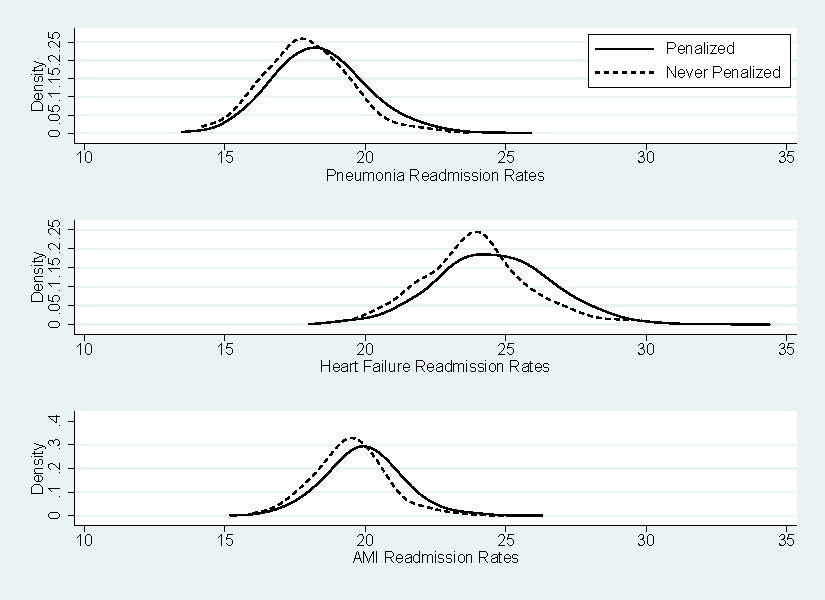
\includegraphics[scale=1]{Readmit_Graphs.pdf}
}
\setlength{\captionmargin}{.5 \textwidth} \addtolength{\captionmargin}{-.5\wd\gfxbox}
\begin{figure}[htbp!]
\centering
\caption{Pre-HRRP/HVBP Readmission Rates}
\label{fig:pre_readmits}
\usebox{\gfxbox}
\par
\begin{minipage}{\wd\gfxbox}
\footnotesize
Notes:  Kernel density estimates for readmission rates prior to HRRP/HVBP among hospitals ultimately penalized versus those not penalized. Readmission rates reflect reported rates in 2010 and 2011, which are constructed from rates in 2006-2009 and 2007-2010, respectively.
\end{minipage}
\end{figure}
\newpage


\section*{Tables}


\savebox{\gfxbox}{
\footnotesize
\begin{tabular}{ccccccc}
\hline \hline
%\multicolumn{9}{c}{}\\
Fiscal & Sample 	&  Payment $\$$				& Medicare   & Medicaid  	& Other & Percent \\
Year   &  Size    	&  Mean (St. Dev.) 				& Discharges    	& Discharges       	& Discharges   & Penalized \\
 \hline
2010 &      1,386		& 	10,729.22   (4,936.50)	 &   4,614.62  &   2,010.11    &  7,898.18  & 0.00  \\
2011 &      1,386		& 	11,602.74   (5,076.45)	&  4,618.93    & 1,960.05    &  7,892.21  & 0.00   \\
2012 & 	1,386 		& 	12,079.46   (5,477.37) 	  &  4,493.31  &  1,810.27   &   8,019.04  & 0.32   \\
2013 & 	1,386		& 	12,668.44   (5,567.76)	  & 4,396.32    & 1,783.81    &  7,996.10  & 0.74  \\
2014 & 	1,386		&	12,795.83   (5,444.21)	 &    4,260.43   &   1,726.25  &    7,852.71 & 0.76 \\
2015 &    1,386			& 	13,397.63   (5,921.74)	&    4,311.41   &  1,578.86    &   8,261.74 & 0.79 \\
\hline
Total & 	8,316		& 12,212.22   (5,481.55)	  &    4,449.17   &  1,811.56  &   7,986.67 & 0.43 \\
\hline
\end{tabular}
}
\setlength{\captionmargin}{.5 \textwidth} \addtolength{\captionmargin}{-.5\wd\gfxbox}
\begin{table}[htbp!]
\centering
\caption{Characterization of Research Sample over Time}
\label{tab:summarystats}
\usebox{\gfxbox}
\par
\begin{minipage}{\wd\gfxbox}
\footnotesize
Notes: Balanced panel of hospitals over time between 2010 and 2015.  Payment represents the mean dollar amount paid to a hospital in a year over all acute care admissions.  Penalty is a binary variable for whether the combination of HRRP and HVBP resulted in a net payment reduction. Other discharges denotes all discharges other than Medicare and Medicaid.
\end{minipage}
\end{table}



\newpage
\savebox{\gfxbox}{
\scriptsize
\begin{tabular}{lccc}
\hline \hline
Variable 				& Never 			& Ever  				&   	  \\
		   			&  Penalized    		& Penalized			&    p-value   				\\
 \hline
Log(Payment)			&	9.423	&	9.300	&	0.000	\\
Log(Charge)			&      8.843	&	8.726	& 	0.000	\\
System  Membership      	&	0.768	&	0.784	&	0.352	\\
Non-profit     			&	0.790	&	0.692	&	0.000	\\
Log(Case Mix Index)        	&	0.437	&	0.447	&	0.090	\\
\multicolumn{4}{l}{Local Hospital}\\							
\hspace{0.05in} Monopoly  	&	0.133	&	0.113	&	0.110	\\
\hspace{0.05in} Duopoly    	&	0.282	&	0.156	&	0.000	\\
\hspace{0.05in} Triopoly   	&	0.139	&	0.108	&	0.012	\\
\multicolumn{4}{l}{Market Share}\\							
\hspace{0.05in} Medicare  	&	0.338	&	0.330	&	0.056	\\
\hspace{0.05in} Medicaid    	&	0.110	&	0.125	&	0.000	\\
\hspace{0.05in} Medicare+Medicaid      	&	0.447	&	0.455	&	0.086	\\
\hspace{0.05in} Other     	&	0.553	&	0.545	&	0.086	\\
Total Pop. (1000s)     	&	714	&	1,190	&	0.000	\\
\multicolumn{4}{l}{County Age Distribution}\\							
\hspace{0.05in}[18, 34]      	&	0.240	&	0.239	&	0.504	\\
\hspace{0.05in}[35, 64]   	&	0.393	&	0.393	&	0.947	\\
\hspace{0.05in}$>$65    	&	0.133	&	0.130	&	0.101	\\
\multicolumn{4}{l}{County Race Distribution}\\							
\hspace{0.05in}White     	&	0.795	&	0.734	&	0.000	\\
\hspace{0.05in}Black    	&	0.096	&	0.134	&	0.000	\\
\multicolumn{4}{l}{County Income Distribution}\\							
\hspace{0.05in}$<$ \$50k   	&	0.185	&	0.180	&	0.000	\\
\hspace{0.05in}[\$50k, 75k]   	&	0.126	&	0.123	&	0.000	\\
\hspace{0.05in}[\$100k, 150k]       	&	0.132	&	0.132	&	0.820	\\
\hspace{0.05in}$>$ \$150k   	&	0.095	&	0.101	&	0.007	\\
\multicolumn{4}{l}{County Education Distribution}\\							
\hspace{0.05in}High School Only  	&	0.270	&	0.270	&	0.925	\\
\hspace{0.05in}Bachelor's Only    	&	0.197	&	0.191	&	0.005	\\
\hline
\end{tabular}
}
\setlength{\captionmargin}{.5 \textwidth} \addtolength{\captionmargin}{-.5\wd\gfxbox}
\begin{table}[htbp!]
\centering
\caption{Hospital Characteristics by Penalties}
\label{tab:bypenalty}
\usebox{\gfxbox}
\par
\begin{minipage}{\wd\gfxbox}
\footnotesize
Notes:  $n=8,316$ Summary statistics are split by whether a hospital is ever observed to receive a net penalty in 2012-2015. Payment represents the mean dollar amount paid to a hospital in a year over all acute care admissions.   County level characteristics are from the American Community Survey.
\end{minipage}
\end{table}

\newpage

\savebox{\gfxbox}{
\scriptsize
\begin{tabular}{llllll}
\hline\hline
 							& Log Mean		& Log Mean			& Log Medicaid 	   	& Log Medicare   	& Log Other  			\\
							& Payment		& Net Charge		& Discharges      	& Discharges  		& Discharges        	\\
\hline
\multicolumn{6}{l}{Full Sample: $n=8,316$} \\
\hspace{0.05in}OLS			  				&	-0.061***   &	-0.049***		&	0.220***		&	0.094***		&	0.069***	\\
											&	(0.015)		&	(0.018)			&	(0.045)			&	(0.026)			&	(0.022) 	\\
\hspace{0.05in}OLS	+ Hospital FE			&	0.014***	&	0.008			&	-0.045**		&	-0.027***		&	-0.004		\\
											&	(0.005)		&	(0.008)			&	(0.021)			&	(0.007)			&	(0.011)		\\
\hspace{0.05in}OLS	+ Hospital FE +			&	0.010*		&	0.019**			&	-0.038			&	-0.026***		&	-0.011		\\
\hspace{0.1in} + Ever Penalized Trends		&	(0.005)		&	(0.008)			&	(0.023)			&	(0.007)			&	(0.012)		\\
\hspace{0.1in} Differential Trend p-value 	&	[0.498]		&	[0.041]			&	[0.250]			&	[0.005]			&	[0.446]		\\
\hspace{0.05in}OLS	+ Hospital FE +	IV		&	0.037**		&	-0.048**		&	-0.087			&	-0.031			&	0.033		\\
											&	(0.014)		&	(0.024)			&	(0.058)			&	(0.020)			&	(0.028)		\\
\hspace{0.1in} OverID p-value			 	&	[0.899]		&	[0.511]			&	[0.875]			&	[0.990]			&	[0.924]		\\
\hline
\multicolumn{6}{l}{Restricted Sample: $n=6,954$} \\
\hspace{0.05in}OLS			  				&	-0.073***	&	-0.077***		&	0.305***		&	0.150***		&	0.113***	\\
											&	(0.021)		&	(0.025)			&	(0.062)			&	(0.036)			&	(0.030)		\\
\hspace{0.05in}OLS	+ Hospital FE			&	0.018***	&	0.002			&	-0.029			&	-0.024***		&	0.001		\\
											&	(0.007)		&	(0.011)			&	(0.029)			&	(0.009)			&	(0.012)		\\
\hspace{0.05in}OLS	+ Hospital FE +			&	0.012		&	0.025**			&	0.001			&	-0.020**		&	-0.012		\\
\hspace{0.1in} + Ever Penalized Trends		&	(0.008)		&	(0.012)			&	(0.035)			&	(0.010)			&	(0.014)		\\
\hspace{0.1in} Differential Trend p-value 	&	[0.903]		&	[0.026]			&	[0.142]			&	[0.002]			&	[0.469]		\\
\hspace{0.05in}OLS	+ Hospital FE +	IV		&	0.029**		&	-0.049**		&	-0.095*			&	-0.032*			&	0.031		\\
											&	(0.013)		&	(0.022)			&	(0.051)			&	(0.018)			&	(0.024)		\\
\hspace{0.1in} OverID p-value			 	&	[0.941]		&	[0.414]			&	[0.949]			&	[0.877]			&	[0.717]		\\
\hline
\end{tabular}
}
\setlength{\captionmargin}{.5 \textwidth} \addtolength{\captionmargin}{-.5\wd\gfxbox}
\begin{table}[htbp!]
\centering
\caption{Baseline Results}
\label{tab:baselineresults}
\usebox{\gfxbox}
\par
\begin{minipage}{\wd\gfxbox}
\footnotesize
Notes: Each point estimate represents the estimated coefficient on a binary variable for whether or not a hospital received a net penalty in a given year.  All regressions include year fixed effects and other hospital level controls include bed count, number of nurses, and number of other non-medical staff.  Market power variables are constructed using the overall hospital service area.  Large market is a binary variable for a hospital in the top half of the market size distribution.  In cases in which independent variables are missing, we recode them and control for missing variable indicators to ensure a balanced panel.  The restricted sample includes only hospitals that were never penalized and those first penalized prior to 2014.  Differential trend p-value is from the F-test that all year dummy interactions with ever penalized are zero.  OverID p-value is from the test that the interaction between a 2011 dummy and ever-penalized is zero in the second stage.  Standard errors are clustered at the hospital level.  *** p-value$<$0.01, ** p-value$<$0.05, * p-value$<$0.1.
\end{minipage}
\end{table}




%%%%%%%%%%%%%%%%%%%%%%%%%%%%%%%%%%%%% The Old Table 3
%\savebox{\gfxbox}{
%\scriptsize
%\begin{tabular}{llllll}
%\hline\hline
% 			& Log Mean		& Log Mean			& Log Medicaid 	   	& Log Medicare   		& Log Other  			\\
%			& Payment		& 	Net Charge		& Discharges      		& Discharges       	& Discharges        	\\
%\hline
%Net Penalty  					&	0.014***	&	0.008	&	-0.045**	&	-0.027***	&	-0.004	\\
%							&	(0.005)	&	(0.008)	&	(0.021)	&	(0.007)	&	(0.011)	\\
%\multicolumn{6}{l}{Hospital Characteristics}\\											
%\hspace{0.15in} Monopoly			&	-0.008	&	0.004	&	-0.025	&	0.003	&	-0.012	\\
%							&	(0.012)	&	(0.011)	&	(0.055)	&	(0.025)	&	(0.029)	\\
%\hspace{0.15in} Duopoly			&	-0.005	&	0.010	&	0.036	&	0.030	&	0.013	\\
%							&	(0.010)	&	-(0.010)	&	(0.044)	&	(0.019)	&	(0.023)	\\
%\hspace{0.15in} Triopoly			&	0.000	&	0.003	&	-0.000	&	0.002	&	0.006	\\
%							&	(0.009)	&	(0.008)	&	(0.039)	&	(0.015)	&	(0.019)	\\
%\hspace{0.10in} Large Market		&	-0.041	&	0.001	&	-0.063	&	0.049**	&	0.179***	\\
%							&	(0.028)	&	(0.013)	&	(0.050)	&	(0.020)	&	(0.043)	\\
%\hspace{0.10in} Any Teaching		&	-0.018	&	-0.022	&	-0.047	&	-0.021	&	-0.013	\\
%							&	(0.012)	&	(0.014)	&	(0.039)	&	(0.016)	&	(0.022)	\\
%\hspace{0.10in} Major Teaching		&	0.003	&	-0.001	&	0.008	&	0.009	&	0.011	\\
%							&	(0.006)	&	(0.004)	&	(0.026)	&	(0.010)	&	(0.012)	\\
%\hspace{0.10in} System			&	0.019	&	-0.002	&	-0.091**	&	-0.066***	&	-0.083***	\\
%							&	(0.015)	&	(0.011)	&	(0.041)	&	(0.019)	&	(0.020)	\\
%\hspace{0.10in} Nonprofit			&	0.020 &	-0.009	&	0.073	&	0.036	&	0.016	\\
%							&	(0.026)	&	(0.016)	&	(0.058)	&	(0.028)	&	(0.032)	\\
%\multicolumn{6}{l}{County Age Share}\\											
%\hspace{0.1in}[18,34]			&	-1.132*	&	-0.896*	&	2.902	&	-3.163***	&	-1.418	\\
%							&	(0.681)	&	(0.543)	&	(2.327)	&	(0.853)	&	(0.880)	\\
%\hspace{0.1in}[35,64]			&	-0.402	&	-1.182*	&	2.923	&	-3.428***	&	-0.044	\\
%							&	(0.910)&	(0.656)	&	(2.781)	&	(1.171)	&	(1.295)	\\
%\hspace{0.1in} $>$64			&	-0.488	&	0.281	&	-1.440	&	0.361	&	-0.838	\\
%							&	(0.797)	&	(0.671)	&	(2.765)	&	(1.245)	&	(1.359)	\\
%\multicolumn{6}{l}{County Share in Income Group}\\											
%\hspace{0.1in} 50k-75k			&	-0.288	&	-0.034	&	1.518	&	-0.173	&	0.420	\\
%							&	(0.386)	&	(0.286)	&	(1.439)	&	(0.548)	&	(0.790)	\\
%\hspace{0.1in} 75k-100k			&	-0.279	&	0.649*	&	0.281	&	-0.319	&	-0.286	\\
%							&	(0.479)	&	(0.352)	&	(1.736)	&	(0.623)	&	(0.791)	\\
%\hspace{0.1in} 100k-150k			&	-0.736	&	0.290	&	-1.847	&	-0.017	&	0.072	\\
%							&	(0.457)	&	(0.313)	&	(1.533)	&	(0.625)	&	(0.776)	\\
%\hspace{0.1in}$>$150k			&	0.891**	&	-0.139	&	0.814	&	0.997*	&	-1.767***	\\
%							&	(0.402)	&	(0.314)	&	(1.375)	&	(0.511)	&	(0.671)	\\
%\hline
%\end{tabular}
%}
%\setlength{\captionmargin}{.5 \textwidth} \addtolength{\captionmargin}{-.5\wd\gfxbox}
%\begin{table}[htbp!]
%\centering
%\caption{Baseline Results}
%\label{tab:baselineresults}
%\usebox{\gfxbox}
%\par
%\begin{minipage}{\wd\gfxbox}
%\footnotesize
%Notes: $n=8,316$.  All regressions include hospital and year fixed effects, and other hospital level controls include bed count, number of nurses, and number of other non-medical staff.  Market power variables are constructed using the overall hospital service area.  Large market is a binary variable for a hospital in the top half of the market size distribution.  In cases in which independent variables are missing, we recode them and control for missing variable indicators to ensure a balanced panel.  Standard errors are clustered at the hospital level.  *** p-value$<$0.01, ** p-value$<$0.05, * p-value$<$0.1.
%\end{minipage}
%\end{table}






\newpage
\savebox{\gfxbox}{
\scriptsize
\begin{tabular}{lc|lllll}
\hline\hline
Penalty 		& Mean Penalty Per Medicare 	& Log Mean		& Log Mean			& Log Medicaid 	   	& Log Medicare   		& Log Other  			\\
Quartile		&  Discharge [Range]	& Payment		& 	Net Charge		& Discharges      		& Discharges       	& Discharges        	\\
\hline
\multicolumn{7}{c}{Reference Category $=$ No Penalty or Bonus} \\

1	&$\$$6.00 &	0.004	&	0.01	&	-0.007	&	0.001	&	0.006	\\
	&[$\$$0.01, $\$$12.59] &	(0.006)	&	(0.009)	&	(0.025)	&	(0.008)	&	(0.012)	\\
2	&$\$$20.21&	0.020***	&	0.007	&	-0.053**	&	-0.018**	&	0.005	\\
	&[$\$$12.59, $\$$29.08]&	(0.006)	&	(0.009)	&	(0.024)	&	(0.008)	&	(0.013)	\\
3& $\$$41.77	&	0.014**	&	0.001	&	-0.061**	&	-0.035***	&	-0.006	\\
	& [$\$$29.15, $\$$57.06]&	(0.006)	&	(0.011)	&	(0.027)	&	(0.009)	&	(0.013)	\\
4& $\$$94.25&	0.024***	&	0.016	&	-0.085***	&	-0.085***	&	-0.036**	\\
	& [$\$$57.10, $\$$291.60]&	(0.008)	&	(0.013)	&	(0.030)	&	(0.012)	&	(0.015)	\\
\hline
\end{tabular}
}
\setlength{\captionmargin}{.5 \textwidth} \addtolength{\captionmargin}{-.5\wd\gfxbox}
\begin{table}[htbp!]
\centering
\caption{Intensive Margin Results}
\label{tab:int}
\usebox{\gfxbox}
\par
\begin{minipage}{\wd\gfxbox}
\footnotesize
Notes: $n=8,316$.  Results derived from breaking the size of the per Medicare discharge penalty into quartiles, with the omitted category as those hospitals receiving no penalty or a bonus.  All regressions include hospital and year fixed effects, and other hospital level controls include bed count, number of nurses, and number of other non-medical staff.  Market power variables are constructed using the overall hospital service area.  In cases in which independent variables are missing, we recode them and control for missing variable indicators to ensure a balanced panel.  Standard errors are clustered at the hospital level.   *** p-value$<$0.01, ** p-value$<$0.05, * p-value$<$0.1.
\end{minipage}
\end{table}


\savebox{\gfxbox}{
\footnotesize
\begin{tabular}{ccccccc}
\hline	
\hline
 							& Nervous  	& Respiratory  	 & Circulatory    & Musculoskeletal   		& Labor and & Neonatal \\
							&  System		&  System      	&  System     	&  System        			& Delivery   &	\\
\hline
Net Penalty 					& 0.021***		&	0.001 	&	0.019**	&	0.004	&	-0.001	&	0.016	\\
							& (0.010)		&	(0.011)	&	(0.008)	&	(0.007)	&	(0.005)	&	(0.010)	\\
\hline
n							& 1,410		&	1,758 	&	2,754  	&	3,060  	&	5,226	&	3,204	\\
Mean 						&13,762.86	&	12,015.13	&	13,071.17	&	12,981.58	&	11,308.56	&	8,911.19	\\
\hline
\end{tabular}
}
\setlength{\captionmargin}{.5 \textwidth} \addtolength{\captionmargin}{-.5\wd\gfxbox}
\begin{table}[htbp!]
\centering
\caption{Log Payments for Condition Specific Admissions}
\label{tab:eachcondition}
\usebox{\gfxbox}
\par
\begin{minipage}{\wd\gfxbox}
\footnotesize
Notes: All regressions include hospital and year fixed effects.  The dependent variable is the log of average payments for each associated acute care admission.  Further controls include those in our baseline specification for mean payments.  In cases in which independent variables are missing, we recode them and control for missing variable indicators to ensure a balanced panel.  Standard errors are clustered at the hospital level.  We restrict the sample to include at least 25 admissions per hospital per year.  *** p-value$<$0.01, ** p-value$<$0.05, * p-value$<$0.1.
\end{minipage}
\end{table}



\newpage
\savebox{\gfxbox}{
\footnotesize
\begin{tabular}{llllll}
\hline	
\hline
 			& Log Mean 				& Log Mean			& Log Medicaid 	   	& Log Medicare   		& Log Other  			\\
			& Payment		& 	Net Charge	& Discharges      		& Discharges       	& Discharges    \\
	\hline
											
\multicolumn{6}{c}{1. Hospital, Year, and County Fixed Effects} 											\\
\hline											
Net Penalty 	&	0.015***	&	0.009	&	-0.048**	&	-0.027***	&	-0.003	\\
			&	(0.005)	&	(0.008)	&	(0.022)	&	(0.007)	&	(0.011)	\\
\hline											
\multicolumn{6}{c}{2. Controlling for Medicaid Expansion States} 											\\
\hline											
Net Penalty 	&	0.014***	&	0.008	&	-0.044**	&	-0.027***	&	-0.005	\\
			&	(0.005)	&	(0.008)	&	(0.021)	&	(0.007)	&	(0.010)	\\
\hline											
\multicolumn{6}{c}{3. Controlling for Overall HCAHPS Hospital Rating} 											\\
\hline											
Net Penalty 	&	0.014***	&	0.008	&	-0.045**	&	-0.026***	&	-0.003	\\
			&	(0.005)	&	(0.008)	&	(0.021)	&	(0.007)	&	(0.010)	\\
\hline											
\multicolumn{6}{c}{4. Dropping Fiscal 2012} 											\\
\hline											
Net Penalty 	&	0.012**	&	0.010	&	-0.045*	&	-0.028***	&	-0.007	\\
			&(0.005)		&	(0.009)		&(0.023)		&(0.007)	&	(0.012)	\\
\hline											
\multicolumn{6}{c}{5. Controlling for Case Mix} 		\\								
\hline											
Net Penalty 	&	0.014***	&	0.004	&	-0.044**	&	-0.026***	&	-0.005	\\
				&(0.005)		&	(0.008)		&(0.021)		&(0.007)	&	(0.011)	\\
\hline

\end{tabular}
}
\setlength{\captionmargin}{.5 \textwidth} \addtolength{\captionmargin}{-.5\wd\gfxbox}
\begin{table}[htbp!]
\centering
\caption{Robustness Checks}
\label{tab:robustness}
\usebox{\gfxbox}
\par
\begin{minipage}{\wd\gfxbox}
\footnotesize
Notes: Further controls include those in our baseline specification for mean payments.  The p-value in the first row of results is in reference to the null hypothesis that trends in the outcome of interest are the same between ever-penalized and never-penalized hospitals conditional on the model covariates.  In cases in which independent variables are missing, we recode them and control for missing variable indicators to ensure a balanced panel.  Standard errors are clustered at the hospital level.   *** p-value$<$0.01, ** p-value$<$0.05, * p-value$<$0.1.
\end{minipage}
\end{table}


\newpage
\savebox{\gfxbox}{
\footnotesize
\begin{tabular}{lllllll}
\hline\hline
 				&  Patient-Level & Log & Profit Index 	& Average DRG & Average  & Log Cost per     	\\
 				& 	Readmission & Charge & 			& Weight 		& LOS & 	Discharge 	\\
\hline
\hline							
Net Penalty  		& -0.001 & 0.004 &	0.002	&	0.004	& 	0.015  & -0.001 \\
				& (0.001) & (0.004) &	(0.001)	&	(0.004)	&	(0.012) & (0.001)  	\\
n				& 3,345,641 & 8,316 & 8,316& 8,316 & 8,316 & 8,238  \\
															
\hline
\end{tabular}
}
\setlength{\captionmargin}{.5 \textwidth} \addtolength{\captionmargin}{-.5\wd\gfxbox}
\begin{table}[htbp!]
\centering
\caption{Changes in Quality or Treatment Intensity}
\label{tab:other_results}
\usebox{\gfxbox}
\par
\begin{minipage}{\wd\gfxbox}
\footnotesize
Notes: All regressions include hospital and year fixed effects, and other hospital level controls include bed count, number of nurses, and number of other non-medical staff. In cases in which independent variables are missing, we recode them and control for missing variable indicators to ensure a balanced panel.  Standard errors are clustered at the hospital level.   *** p-value$<$0.01, ** p-value$<$0.05, * p-value$<$0.1.
\end{minipage}
\end{table}

\newpage
\savebox{\gfxbox}{
\footnotesize
\begin{tabular}{llllll}
\hline	
\hline
 			& Log Mean			& Log Mean				& Log Medicaid 	   	& Log Medicare   		& Log Other  			\\
			& Payment			& Net Charge				& Discharges      		& Discharges       	& Discharges    \\
	\hline
\multicolumn{6}{c}{Non-profit Hospitals}\\											
\hline											
Net Penalty 	&	0.015***	&	0.008	&	-0.046*	&	-0.029***	&	-0.011	\\
			&	(0.005)	&	(0.009)	&	(0.024)	&	(0.007)	&	(0.012)	\\
\hline											
\multicolumn{6}{c}{Non-Profit Hospitals with Penalty Specific Trends} 											\\
						\hline					
Net Penalty 	&	0.012**	&	0.015*	&	-0.039	&	-0.023***	&	-0.015	\\
			&	(0.005)	&	(0.009)	&	(0.026)	&	(0.007)	&	(0.014)	\\
p-value & 0.805 & 0.205 & 0.241 & 0.001 & 0.849 \\
\hline											
\multicolumn{6}{c}{For-profit Hospitals}\\											
\hline											
Net Penalty 	&	0.020	&	0.023	&	-0.018	&	-0.008	&	0.026	\\
			&	(0.014)	&	(0.021)	&	(0.050)	&	(0.018)	&	(0.020)	\\
\hline											
\multicolumn{6}{c}{For-Profit Hospitals with Penalty Specific Trends} 											\\
\hline											
Net Penalty	&	0.011	&	0.043*	&	0.002	&	-0.028	&	0.007	\\
			&	(0.014)	&	(0.023)	&	(0.050)	&	(0.017)	&	(0.020)	\\
p-value & 0.417 & 0.025 & 0.885 & 0.013 & 0.003 \\
\hline
\end{tabular}
}
\setlength{\captionmargin}{.5 \textwidth} \addtolength{\captionmargin}{-.5\wd\gfxbox}
\begin{table}[htbp!]
\centering
\caption{Results by Profit Status}
\label{tab:byprofit}
\usebox{\gfxbox}
\par
\begin{minipage}{\wd\gfxbox}
\footnotesize
Notes: All regressions include hospital and year fixed effects.  Further controls include those in our baseline specification for mean payments.  The p-values are in reference to the null hypothesis that trends in the outcome of interest are the same between ever-penalized and never-penalized hospitals conditional on the model covariates.  In cases in which independent variables are missing, we recode them and control for missing variable indicators to ensure a balanced panel.  Standard errors are clustered at the hospital level.   *** p-value$<$0.01, ** p-value$<$0.05, * p-value$<$0.1.
\end{minipage}
\end{table}








\newpage
\savebox{\gfxbox}{
\footnotesize
\begin{tabular}{lll}
\hline	
 		& Log Mean & Log Mean   				 \\
		& Payment & Net Charge\\
\hline
Net Penalty				&	0.039***	&	0.043***	\\
						&	(0.010)	&	(0.013)	\\
\hspace{0.1in}* Public Share 2 	&	-0.020*	&	-0.014	\\
						&	(0.012)	&	(0.014)	\\
\hspace{0.1in}* Public Share 3	&	-0.033**	&	-0.043***	\\
						&	(0.013)	&	(0.015)	\\
\hspace{0.1in}* Public Share 4	&	-0.044***	&	-0.070***	\\
						&	(0.013)	&	(0.016)	\\
Public Share 2				&	0.007	&	0.049***	\\
						&	(0.010)	&	(0.013)	\\
Public Share 3				&	0.016	&	0.087***	\\
						&	(0.011)	&	(0.016)	\\
Public Share 4				&	0.023*	&	0.157***	\\
						&	(0.012)	&	(0.018)	\\
\hline
\end{tabular}
}
\setlength{\captionmargin}{.5 \textwidth} \addtolength{\captionmargin}{-.5\wd\gfxbox}
\begin{table}[htbp!]
\centering
\caption{Triple Differences by Public Share}
\label{tab:publicshare}
\usebox{\gfxbox}
\par
\begin{minipage}{\wd\gfxbox}
\footnotesize
Notes: All regressions include hospital and year fixed effects.  Further controls include those in our baseline specification for mean payments.  The share of a hospital's patients insured by the public sector is broken into quartiles and interacted with penalty variables.  In cases in which independent variables are missing, we recode them and control for missing variable indicators to ensure a balanced panel.  Standard errors are clustered at the hospital level.  We restrict the sample to include at least 25 admissions per hospital per year.  *** p-value$<$0.01, ** p-value$<$0.05, * p-value$<$0.1.
\end{minipage}
\end{table}




\newpage
\savebox{\gfxbox}{
\footnotesize
\begin{tabular}{llllll}
\hline	
\hline
 & Log Mean 				& Log Mean			& Log Medicaid 	   	& Log Medicare   		& Log Other  			\\
			& Payment		& 	Net Charge	& Discharges      		& Discharges       	& Discharges    \\
\hline
\multicolumn{6}{c}{Hospitals Integrated Vertically with Physician Groups Prior to 2012} 											\\
\hline											
Net Penalty 	&	0.023***		&	0.017***	&	-0.036	&	-0.026**	&	0.008	\\
			&	(0.008)		&	(0.006)		&(0.032)		&(0.009)	&	(0.016)	\\
			\hline
\multicolumn{6}{c}{Hospitals Never Observed to be Vertically Integrated with a Physician Group} 											\\
\hline											
Net Penalty 	&	0.008		&	0.021***	&	-0.063**	&	-0.024**	&	-0.005	\\
			&	(0.007)		&	(0.012)		&(0.031)		&(0.010)	&	(0.015)	\\
			\hline
\end{tabular}
}
\setlength{\captionmargin}{.5 \textwidth} \addtolength{\captionmargin}{-.5\wd\gfxbox}
\begin{table}[htbp!]
\centering
\caption{Vertical Integration and Penalties}
\label{tab:VI}
\usebox{\gfxbox}
\par
\begin{minipage}{\wd\gfxbox}
\footnotesize
Notes: Empirical models are identical to those in Table \ref{tab:baselineresults}.  Standard errors are clustered at the hospital level.  *** p-value$<$0.01, ** p-value$<$0.05, * p-value$<$0.1.
\end{minipage}
\end{table}



















\end{document}
